\begin{abstract}
Abstract. In this essay we are giving an overview of our work on fuzzy rules and similarities originally motivated by Peter H\'{a}jek's teaching and work. Our main starting points are Peter's visions of fuzzy logic in narrow sense and understanding of fuzzy values as a comparative notion of truth. Fuzzy logic in narrow sense is in our work reflected by formal models of fuzzy logic programming and similarities. Comparative notion of truth led us to understand fuzzy values as degree of user preference. As far as mathematical fuzzification of a domain can lead to several possible models, computer science application needs can help to fix one. In this essay we overview our work (originally published with several coauthors) on models of fuzzy logic programming and its connection to generalized annotated programs and similarity reasoning; on fuzzy inductive logic programming; application to user preference learning and querying; applications to web information extraction and web semantization.
\end{abstract}


\section{Introduction, motivation, problems.}

     Origins of fuzzy sets is connected to seminal work of L. A. Zadeh \cite{Z}. original motivation was image processing where different grades of shade of image pixel were first practical examples of fuzzy sets (see e.g. picture \ref{fig:img1}a \cite{p1a}). Fuzzy set theory has developed rapidly with main applications in control (see e.g. pictures \ref{fig:img1}b and \ref{fig:img1}c \cite{p1bc}, where rules for an inverted pendulum \ref{fig:img1}b are trained using fuzzy sets ,e.g. \ref{fig:img1}c). 


\begin{figure}[htbp]
	\centering
		\includegraphics[width=1.00\textwidth]{img/img1}
	\label{fig:img1}
	\caption{(a, b, c)}
\end{figure}



     Another motivation for fuzzy sets was modeling vague concepts like tall, young, etc. Many applications needed formal models. Here is the first contribution of Petr H\'{a}jek. In \cite{Ha2} he further develops Zadeh's terms "fuzzy logic in broad or wide and narrow sense." In broad sense the term fuzzy logic has been used as synonymous with fuzzy set theory and its applications. In difference to Zadeh, which understood the emerging narrow sense fuzzy logic as a theory of approximate reasoning based on many valued logic, H\'{a}jek claims "... a logician will first study classical logical questions on completeness, decidability, complexity etc. of the symbolic calculi in question and then try to reduce question of Zadeh's agenda to questions of deduction as far as possible.  This is the approach in monograph of Petr H\'{a}jek \cite{Ha}. 
     
     Petr H\'{a}jek introduced fuzzy logic in narrow sense as a mathematical theory of many valued logic. First contribution was done by J. Pavelka in \cite{P} where he used graded statements (propositions), e.g.
\begin{displaymath}
p. 0,5\ \ \ p \rightarrow q. 0,7
\end{displaymath}
to development of an axiomatic system of Lukasiewicz logic. 
     
     Basic development by Petr H\'{a}jek \cite{Ha} was interested in axiomatization of 1-tautologies of various fuzzy logics. Just to motivate our view of this approach, let us notice that classical 0-1 tautology 
\begin{equation} \label{eq:taut1}
(\varphi\rightarrow(\psi\rightarrow\chi))\rightarrow((\varphi\rightarrow\psi)\rightarrow(\psi\rightarrow\chi))
\end{equation}
is no more a tautology even in a 3 valued logic. This has P. H\'{a}jek to the study of metamathematics of fuzzy logic, which is more detailed presented in some papers of this volume. This concerns especially introduction and study of so called Basic Logic BL, where (\ref{eq:taut1}) is not provable and there are some BL axioms replacing this form of composed implications, e.g. 
\begin{displaymath}
(\varphi\rightarrow\psi)\rightarrow((\psi\rightarrow\chi)\rightarrow(\varphi\rightarrow\chi))
\end{displaymath}

     For tuning real world applications to data, and moreover online with response in a second, it is hard to follow this way (to work with axiomatic systems). 

     Nevertheless our main motivation came from attending lectures of Petr H\'{a}jek on fuzzy logic \cite{HaTUW}, where he introduced fuzzy values as a comparative notion of truth (see also \cite{Ha2}). This was quite well in concordance to different representation of preferences in computer science applications. There are various ways of graphical representation of preference, importance, relevance etc. For user feedback we can use colors as in traffic lights (2a), different smiley's (2b), stars (2c) or sliders (2d).

\begin{figure}[htbp]
	\centering
		\includegraphics[width=1.00\textwidth]{img/img2}
	\label{fig:img2}
	\caption{(a, b, c, d)}
\end{figure}
 


For representation of results we can use Google like graphics (3d) and mnemonics of top-down and let-right reading, enhanced by font size (3b). Another possibility thumbs up/down mnemonic (3c) and understanding colors in geographic maps, the higher terrain the better answer   (\cite{JVKH}).

\begin{figure}[htbp]
	\centering
		\includegraphics[width=1.00\textwidth]{img/img3}
	\label{fig:img3}
	\caption{(a, b, c, d)}
\end{figure}

 

     To resume our starting point, these were computer science motivated problems with a small number of truth values (usually 7+-2), data intensive, with adaptation to different users (although in formal models we often use [0,1] interval).
     
\section{Formal models}

For some approaches we have developed formal models.

\subsection{Fuzzy logic programming versus fuzzy resolution.}
     In fuzzy logic programming we have to decide whether rules are implications or clauses, where my deduction procedure is resolution based refutation or database querying. We have studied both approaches. 
     
     In \cite{FSS} we have developed the implication rules, database querying approach. Having 
\begin{displaymath}
p. 0,5\ \ \ p\rightarrow q. 0,7	
\end{displaymath}
and truth function of $\rightarrow$ is an implicator $I:[0,1] \rightarrow [0,1]$ the result q can be deduced by many valued modus ponens with truth at least $C_I(0,5;\ 0,7)$, where $C_I$ is a residual conjunctor to I. For such approach we have proved correctness of fuzzy logic programming (every computed answer is correct) and approximate completeness (every correct answer can be arbitrarily precisely computed). More a fixed point theory was developed too. 
     
     In real world situation, both for user feedback and for query results presentation, we need finite valued fuzzy logic. More over a very low finite number of values. This was already used by psychologist Rensis Likert (see \cite{Li}). Moreover, "Often five ordered response levels are used, although many psychometricians advocate using seven or nine levels; a recent empirical study found that a 5- or 7- point scale may produce slightly higher mean scores relative to the highest possible attainable score, compared to those produced from a 10-point scale, and this difference was statistically significant (see \cite{Li})". This is also a common practice when refereeing papers, usually 7 values range from strong accept to strong reject. 
     
     This was studied in \cite{KLV}, where results of \cite{FSS} where extended for conjunctor which are results of rounding t-norms to a finite scale. Note that rounding a conjunctor C upwards (in x axis to n values, in y axis to m values and in result z axis to k values) gives a conjunctor $C_{n,m}^{k}$ which need not be associative nor commutative (rounding upwards makes these conjunctors left continuous). Our theory of fuzzy logic programming was extended also to this case. 
     
     In practical application it often comes to a situation that user preferences are aggregated from particular objectives, The situation is similar as in light athletic decathlon. Here individual achievements of an athlete are first converted to point (a fuzzy degree usually between 0 and 1000) and then summed up (fuzzy aggregation without normalization). See e.g. results of a race in G\"{o}tzis on 27.5.2001 where R. Sebrle established  first WR  above 9000 points (Fig.~4). %\ref{fig:img4}).

\begin{figure}[htbp]
	\centering
		\includegraphics[width=1.00\textwidth]{img/img4}
	\label{fig:img4}
	\caption{Athletic decathlon -- G\"{o}tzis on 27.5.2001}
\end{figure}


Also in web shops and other user decision making similar phenomena appear. Namely, it can happen that even if having similar objectives one can have different weights for aggregation, or different users can have just opposite directions of preference. 

     For such situations, we have developed a model of fuzzy logic programming where fuzzy aggregations can appear in the body of rule. Such a rule can have form (in graded Prolog notation)
\begin{displaymath}
H\leftarrow @(B_1,...,B_n).r	
\end{displaymath}
We have also showed in \cite{KLV} that these are, in a sense, isomorphic to rules of GAP-Generalized annotated programs (with crisp $\leftarrow$ and \&)
\begin{displaymath}
H:@(b_1,...,b_n)\leftarrow B_1:b_1\&...\&,B_n:b_n	
\end{displaymath} 
and procedural and declarative semantic are also in good connection (for more details see \cite{KLV}). 

\begin{figure}[htbp]
	\centering
		\includegraphics[width=1.00\textwidth]{img/good_price}
	\label{fig:good_price}
	\caption{}
\end{figure}

     Concerning fuzzy resolution, we consider a rule to a clause so instead of $H \leftarrow B$ we write $H \vee \neg B$ and deduction is a refutation process initialized by $\neg H$. We have studied this problem in \cite{SV} in a more general setting, namely graded many valued resolution. This means, having
\begin{displaymath}
(A \vee B).x \ \ \  and \ \ \  (\neg A \vee C).y
\end{displaymath}
We are looking for a function calculating 
\begin{displaymath}
(B \vee C).f_{\vee}(x,y)
\end{displaymath}
Some interesting combination occurred, for more see \cite{SV}. Nevertheless a practical question remains, who will create these clauses, an untrained user probably not. 

\subsection{Fuzzy similarity}

Fuzzy similarity is another phenomenon which important for practical computer science applications. Somebody looking for a resource (web page, document, product, genetic entity, ...) has some requirements, nevertheless it can happen that there are no object fulfilling these requirements. Then a (most) similar resource can make user happy. Similarity is in a sense dual to distance, triangular inequality which is necessary to make a distance metric is dual to transitivity for fuzzy similarity. For a similarity on a domain
\begin{displaymath}
s:A \times A \rightarrow [0,1]
\end{displaymath}
a T-transitivity has form 
\begin{displaymath}
T(s(x,y),s(y,z)) \leq s(x,z)
\end{displaymath}
where T is a t-norm. We say that a space is a T-similarity space if there is a similarity s fulfilling T-transitivity. We say, that a triple
\begin{displaymath}
s(x,y), s(y,z), s(x,z)
\end{displaymath}
is a nontrivial similarity triple, if all there numbers s(x, y), s(y, z) and s(x, z) are mutually different. We have
\\\textbf{Observation.} Assume that similarity s is symmetric and space A is a min-similarity space. Then there are no nontrivial similarity triples in a min-similarity space. 

     Observation is easy if one considers the ordering $s(x, z) < s(x, y) < s(y, z)$ of three different real numbers, then $s(x, z) < min(s(x, y), s(y, z))$. 
     
\begin{figure}[htbp]
	\centering
	\framebox{D O D E L A T  barevny alphas fig}
	\caption{} \label{fig:alpha}
\end{figure}


      Even notice, that the triple min-similarity triple has to have two smaller numbers and only one bigger (see Fig.~\ref{fig:alpha}). This shows that min-similarity spaces have hierarchical structure, $\alpha$-cuts form an equivalence (partition) on A. In real situations this is very often not a case, data are more randomly distributed. A nontrivial similarity triple (Fig.~\ref{fig:triangle}) forces us to consider other t-norms in transitivity than min. If such a triangle is colored in graph terminology we call such a triangle colorful if it contains all tree colors. 

\begin{figure}[htbp]
	\centering
	\framebox{D O D E L A T  barevny triangle}
	\caption{} \label{fig:triangle}
\end{figure}

      This motivates us to following problem. Assume we have Kn a coloring of the complete graph on n vertices by three colors. Is there a colorful triangle? Of course, in general, without any assumption it is not true (see min-transitivity generated colorings). So we can ask, under what conditions on colorings there is a colorful triangle? Note that in a random coloring each triangle is colorful with probability $\frac{2}{9} > 0.2$. This observation is especially useful when considering similarity spaces which are non-metric and similarity distribution is random. For such a spaces (e.g. multimedia, genetic databases) we have developed  in \cite{ESV} an indexing method based on T-similarity, where T is in a sense best similarity under which the space is still a T-similarity space. In \cite{MOV} we have developed the theory of  fuzzy similarity for a general class of  t-norms. 

\section{Tools, Data, Experiments}
     
     In this essay style paper I can confess, that main reason why I have started to study fuzzy induction and/or data mining was a referee, which recommended to reject my paper with an argument that it is not clear where the rules (of my fuzzy logic programming contribution) are coming from. Hence we have developed fuzzy Inductive Logic Programming (FILP) and various descendents. 

\subsection{Mining user preferences and top query answering.}


\begin{figure}[ht]
\begin{minipage}[b]{0.44\hsize}
	\centering
		\includegraphics[width=\hsize]{img/notebook}
\caption{}
\label{fig:notebook}
\end{minipage}
\hspace{0.5cm}
\begin{minipage}[b]{0.5\hsize}
	\centering
		\includegraphics[width=\hsize]{img/aggregation}
\caption{}
\label{fig:aggregation}
\end{minipage}
\end{figure}

     Main motivation for this was learning user preferences from user rating of a set sample set S of objects (see Fig.~\ref{fig:notebook}, mapping $r_u$), where a user interactively evaluates objects by number of stars, without making any comment on item properties. Basis for this is the object attribute representation of data (mapping d in Fig.~\ref{fig:aggregation}), which assigns to each object its data values in the Cartesian product of domains of attributes$\prod_{i=1}^{n}D_{A_{i}}$. The learning task is to find user objectives on particular attributes (fuzzy sets on attribute domains $f_i$) and a fuzzy aggregation function combining these attribute preference degrees. The whole diagram should converge, or at least give good advice for the user. What is a good advice can be measured in several ways, most appropriate for web search is to get best objects (with highest fuzzy degree) first. For this we use Kendal correlation coefficient 
\begin{displaymath}
\tau = \frac{n_c - n_d}{\frac{1}{2}n(n-1)}
\end{displaymath} 
where $n_c$ is the number of concordant pairs, and $n_d$ is the number of discordant pairs in the data set (see \cite{KW}). More on FILP, user preference mining, see \cite{More_on_FILP}.

\begin{figure}[ht]
\begin{minipage}[b]{0.44\hsize}
	\centering
		\includegraphics[width=\hsize]{img/northEast}
\caption{}
\label{fig:northEast}
\end{minipage}
\hspace{0.5cm}
\begin{minipage}[b]{0.5\hsize}
	\centering
		\includegraphics[width=\hsize]{img/index}
\caption{}
\label{fig:index}
\end{minipage}
\end{figure}


     There is another feature in learning user objectives on particular attributes (fuzzy sets on attribute domains $f_i$). This gives an ordering of domains - for user $U_1$ North East direction is better (red rectangle can be objects good in degree at least 0.7) and for user $U_2$ the South West direction is better (blue rectangle can be objects good in degree at least 0.7)  in ordered domain on Fig.~\ref{fig:northEast}. Fuzzy aggregation @ can be glued together from GAP rules like
\begin{quote}
Good\_for\_U1 : 0.7 IF A1 better\_for\_U1 than a AND\\ A2 better\_for\_U1 than b	
\end{quote}
Most of top-k algorithm use ordered approach to data by user preference. But considering different users, this ordering can change and it would be very costly reorder data each time a new user comes. In \cite{FuzzIEEE} we have developed an index structure, which given a fuzzy set can search data starting from best (see Fig.~\ref{fig:index}). 

\subsection{Web information extraction for web semantization}

Web semantization is an idea understanding process of semantization of web resources by third party annotation (as opposed to semantic web idea where it is assumed that web resource creators will annotate their pages by an ontology). Of course annotating web resources by third party is a difficult task. We have tried to make a progress to this task by dividing I to smaller subtasks. First is to consider only tabular product pages and dominantly textual pages. Second idea is to split the task to a domain independent annotation and to domain dependent annotation (here user feedback is necessary, as far we do not have ontology for every domain).

\begin{figure}[ht]
\begin{minipage}[b]{0.4\hsize}
	\centering
		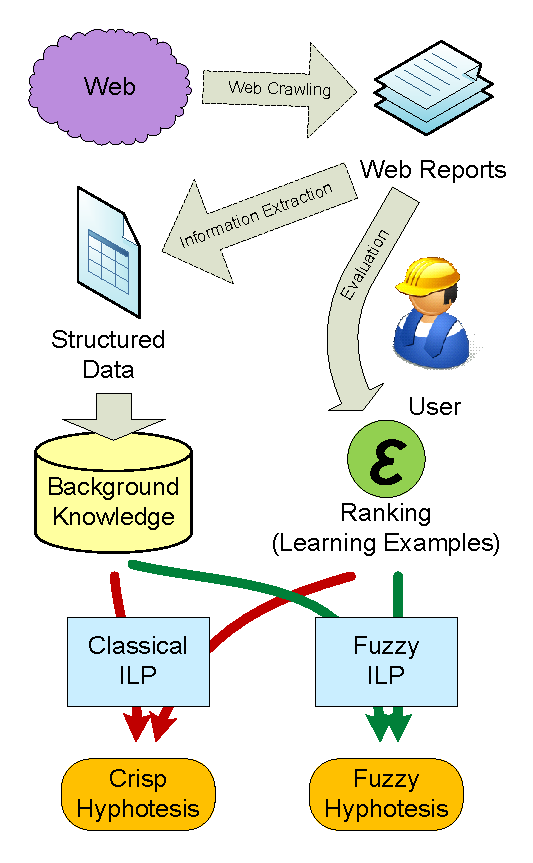
\includegraphics[width=\hsize]{img/schema}
\caption{}
\label{fig:schema}
\end{minipage}
\hspace{0.5cm}
\begin{minipage}[b]{0.5\hsize}
	\centering
		\includegraphics[width=\hsize]{img/mdr}
\caption{}
\label{fig:mdr}
\end{minipage}
\end{figure}


     A strategy for web information extraction of textual pages in depicted in Fig.~\ref{fig:schema}. For domain independent annotation we use a third party linguistic annotator. We use fuzzy ILP for user feedback learning of extracted items. For tabular product pages we use a different approach (Fig.~\ref{fig:mdr}). We parse the HTML structure by a DOM tree and looking for (fuzzy) similarities we can identify Data regions and data records with a quite high accuracy.  For attribute value identification we can make use of an ontology and some regular expressions. If there is no ontology, we can use a heuristics which uses differences in detailed pages. All this projects are part of uncertainty reasoning in the web, especially of fuzzy techniques. 

\section{Conclusions}

In this paper tribute to Petr H\'{a}jek who brought us to fuzzy logic and modeling, we have tried to give an overview of our work in this area and to Petr's influence, especially to consider fuzzy values as a comparative notion of truth which is very well suited for user preference modeling. We have totally ignored contributions of other authors, these can be found in respective papers. 

Concluding we can state that ideas of Petr H\'{a}jek -- both on fuzzy logic in narrow sense and on fuzzy as a comparative notion of truth has brought new insight to many problems, especially to user preference modeling and has led  even to proof of concepts of these ideas based on experimental tools and experiments on real world data. We plan to work in this direction also in the future.

\begin{verbatim}
http://ics.upjs.sk/~gursky/Sk/Publikacie

http://ics.upjs.sk/~horvath/index.php/Research/Publications

http://ics.upjs.sk/~krajci/skola/

http://ics.upjs.sk/~novotnyr/

http://ics.upjs.sk/~vanekova/index.php/Site/Publikacie

pribolova
\end{verbatim}


\begin{thebibliography}{99}
\bibitem{Z} L.A.Zadeh. Fuzzy Sets. Information and control 8 (1965) 338-353
\bibitem{KW} Kendall tau rank correlation coefficient, From Wikipedia, the free encyclopedia
\bibitem{Li} Likert scale, From Wikipedia, the free encyclopedia
\bibitem{ESV} Alan Eckhardt, Tom\'{a}\v{s} Skopal, Peter Vojt\'{a}\v{s} . On fuzzy vs. metric similarity search in complex databases. In FQAS 2009, Springer Verlag 
\bibitem{JVKH} Petr Jencek, Peter Vojtas, Michal Kopecky, Cyril Hoschl. Sociomapping in text retrieval systems. In FQAS 2009, Springer Verlag 
\bibitem{Ha2} Petr H\'{a}jek. Why fuzzy logic? www.logic.at/lvas/185249/Hajek-why-fuzzy.ps
\bibitem{p1a} Airplane picture from http://www.icaen.uiowa.edu/~dip/LECTURE/
\bibitem{p1bc} Inverted pendulum and Fuzzy control system picture From Wikipedia, the free encyclopedia
\bibitem{UPreA} Method for User Preferences Acquisition (tool UPreA), \\http://nazou.fiit.stuba.sk/home/?page=uprea, 
\bibitem{HaTUW} Petr H\'{a}jek, Lectures on fuzzy logic, Technical University Vienna, 1994
\bibitem{Ha} Petr H\'{a}jek. Metamathematics of fuzzy logic, Dordrecht: Kluwer. 1998
\bibitem{Ll} J. W. Lloyd. Foundations of Logic Programming (2nd edition). Springer-Verlag 1987 
\bibitem{P} Pavelka, J., (1979), "On fuzzy logic I, II, III", Zeitschrift fur Math. Logik und Grundlagen der Math, 25: 45-52, 119-134, 447-464
\bibitem{FuzzIEEE} Alan Eckhardt, Jaroslav Pokorn\'{y}, Peter Vojt\'{a}\v{s}: A System Recommending Top-k Objects for Multiple Users Preferences. FUZZ-IEEE 2007: 1-6

\bigskip
50	Alan Eckhardt, Peter Vojt\'{a}\v{s}: Evaluating Natural User Preferences for Selective Retrieval. Web Intelligence/IAT Workshops 2009: 104-107
49		Robert Novotny, Peter Vojt\'{a}\v{s}, Dusan Marusc\'{a}k: Information Extraction from Web Pages. Web Intelligence/IAT Workshops 2009: 121-124
48		Jan Dedek, Peter Vojt\'{a}\v{s}: Fuzzy Classification of Web Reports with Linguistic Text Mining. Web Intelligence/IAT Workshops 2009: 167-170
47		Fernando Bobillo, Paulo Cesar G. da Costa, Claudia d'Amato, Nicola Fanizzi, Francis Fung, Thomas Lukasiewicz, Trevor Martin, Matthias Nickles, Yun Peng, Michael Pool, Pavel Smrz, Peter Vojt\'{a}\v{s}: Proceedings of the Third ISWC Workshop on Uncertainty Reasoning for the Semantic Web Busan, Korea, November 12, 2007 CEUR-WS.org 2008
46		Peter Gursk�, Peter Vojt\'{a}\v{s}: On Top-kSearch with No Random Access Using Small Memory. ADBIS 2008: 97-111
45		Peter Vojt\'{a}\v{s}: Decathlon, Conflicting Objectives and User Preference Querying. DATESO 2008
44		Veronika Vanekov\'{a}, Peter Vojt\'{a}\v{s}: A Description Logic with Concept Instance Ordering and Top-k Restriction. EJC 2008: 139-153
43		Marie Duz�, Anneli Heimb�rger, Takehiro Tokuda, Peter Vojt\'{a}\v{s}, Naofumi Yoshida: Multi-Agent Knowledge Modelling. EJC 2008: 411-428
42		Jan Dedek, Peter Vojt\'{a}\v{s}: Linguistic Extraction for Semantic Annotation. IDC 2008: 85-94
41		Peter Gursk�, Peter Vojt\'{a}\v{s}: Speeding Up the NRA Algorithm. SUM 2008: 243-255
40		Jan Dedek, Alan Eckhardt, Leo Galambos, Peter Vojt\'{a}\v{s}: Discussion on Uncertainty Ontology for Annotation and Reasoning. URSW 2008
39		Alan Eckhardt, Tom\'{a}s Horv\'{a}th, Dusan Marusc\'{a}k, Robert Novotny, Peter Vojt\'{a}\v{s}: Uncertainty Issues and Algorithms in Automating Process Connecting Web and User. URSW (LNCS Vol.) 2008: 207-223
38		Peter Vojt\'{a}\v{s}, Alan Eckhardt: Considering Data-Mining Techniques in User Preference Learning. Web Intelligence/IAT Workshops 2008: 33-36
37		Alan Eckhardt, Jaroslav Pokorn�, Peter Vojt\'{a}\v{s}: Integrating user and group preferences for top-k search from distributed web resources. DEXA Workshops 2007: 317-322
34		Alan Eckhardt, Tom\'{a}s Horv\'{a}th, Peter Vojt\'{a}\v{s}: Learning Different User Profile Annotated Rules for Fuzzy Preference Top-k Querying. SUM 2007: 116-130
33		Alan Eckhardt, Tom\'{a}s Horv\'{a}th, Dusan Marusc\'{a}k, Robert Novotny, Peter Vojt\'{a}\v{s}: Uncertainty Issues in Automating Process Connecting Web and User. URSW 2007
32		Alan Eckhardt, Tom\'{a}s Horv\'{a}th, Peter Vojt\'{a}\v{s}: PHASES: A User Profile Learning Approach for Web Search. Web Intelligence 2007: 780-783
31		Peter Vojt\'{a}\v{s}: EL description logics with aggregation of user preference concepts. EJC 2006: 154-165
30		Tom\'{a}s Horv\'{a}th, Peter Vojt\'{a}\v{s}: Induction of Fuzzy and Annotated Logic Programs. ILP 2006: 260-274
29		Tom\'{a}s Horv\'{a}th, Peter Vojt\'{a}\v{s}: Ordinal Classification with Monotonicity Constraints. Industrial Conference on Data Mining 2006: 217-225
28		Peter Vojt\'{a}\v{s}: EL Description Logic Modeling Querying Web and Learning Imperfect User Preferences. URSW 2006
27		Peter Gursk�, Tom\'{a}s Horv\'{a}th, Robert Novotny, Veronika Vanekov\'{a}, Peter Vojt\'{a}\v{s}: UPRE: User Preference Based Search System. Web Intelligence 2006: 841-844
25		Peter Vojt\'{a}\v{s}: Fuzzy logic as an optimization task. EUSFLAT Conf. 2005: 781-786
24		Tom\'{a}s Horv\'{a}th, Frantisek Sudzina, Peter Vojt\'{a}\v{s}: Mining Rules from Monotone Classification Measuring Impact of Information Systems on Business Competitiveness. BASYS 2004: 451-458
23		Tom\'{a}s Horv\'{a}th, Peter Vojt\'{a}\v{s}: Fuzzy Induction via Generalized Annotated Programs. Fuzzy Days 2004: 419-433
22		Dana Smutn\'{a}, Peter Vojt\'{a}\v{s}: Graded many-valued resolution with aggregation. Fuzzy Sets and Systems 143(1): 157-168 (2004)
21		Stanislav Krajci, Rastislav Lencses, Peter Vojt\'{a}\v{s}: A comparison of fuzzy and annotated logic programming. Fuzzy Sets and Systems 144(1): 173-192 (2004)
20	[MOV] 	Jes�s Medina, Manuel Ojeda-Aciego, Peter Vojt\'{a}\v{s}: Similarity-based unification: a multi-adjoint approach. Fuzzy Sets and Systems 146(1): 43-62 (2004)
18		Jes�s Medina, Manuel Ojeda-Aciego, Agust�n Valverde, Peter Vojt\'{a}\v{s}: Towards Biresiduated Multi-adjoint Logic Programming. CAEPIA 2003: 608-617
17		Stanislav Krajci, Rastislav Lencses, Peter Vojt\'{a}\v{s}: A data model for annotated programs. ADBIS Research Communications 2002: 141-154
16		Stanislav Krajci, Rastislav Lencses, Jes�s Medina, Manuel Ojeda-Aciego, Peter Vojt\'{a}\v{s}: A Similarity-Based Unification Model for Flexible Querying. FQAS 2002: 263-273
15		Stanislav Krajci, Rastislav Lencses, Jes�s Medina, Manuel Ojeda-Aciego, Agust�n Valverde, Peter Vojt\'{a}\v{s}: Non-commutativity and Expressive Deductive Logic Databases. JELIA 2002: 149-160
14		Jes�s Medina, Manuel Ojeda-Aciego, Peter Vojt\'{a}\v{s}: A Multi-Adjoint Approach to Similarity-Based Unification. Electr. Notes Theor. Comput. Sci. 66(5): (2002)
13		Jaroslav Pokorn�, Peter Vojt\'{a}\v{s}: A Data Model for Flexible Querying. ADBIS 2001: 280-293
12		Jes�s Medina, Manuel Ojeda-Aciego, Peter Vojt\'{a}\v{s}: A Procedural Semantics for Multi-adjoint Logic Programming. EPIA 2001: 290-297
11		Jes�s Medina, Manuel Ojeda-Aciego, Peter Vojt\'{a}\v{s}: Similarity-based unification: a multi-adjoint approach. EUSFLAT Conf. 2001: 273-276
10		Jes�s Medina, Manuel Ojeda-Aciego, Peter Vojt\'{a}\v{s}: A Completeness Theorem for Multi-Adjoint Logic Programming. FUZZ-IEEE 2001: 1031-1034
9		Jes�s Medina, Manuel Ojeda-Aciego, Peter Vojt\'{a}\v{s}: A Multi-adjoint Logic Approach to Abductive Reasoning. ICLP 2001: 269-283
8		Jes�s Medina, Manuel Ojeda-Aciego, Peter Vojt\'{a}\v{s}: Multi-adjoint Logic Programming with Continuous Semantics. LPNMR 2001: 351-364
7		Peter Vojt\'{a}\v{s}: Fuzzy logic programming. Fuzzy Sets and Systems 124(3): 361-370 (2001)
6		Peter Vojt\'{a}\v{s}, Zdenek Fabi\'{a}n: Aggregating Similar Witnesses for Flexible Query Answering. FQAS 2000: 220-229
5		Peter Vojt\'{a}\v{s}: Fuzzy logic abduction. EUSFLAT-ESTYLF Joint Conf. 1999: 319-322
\end{thebibliography}
